% Created by tikzDevice version 0.7.0 on 2014-08-02 14:14:01
% !TEX encoding = UTF-8 Unicode
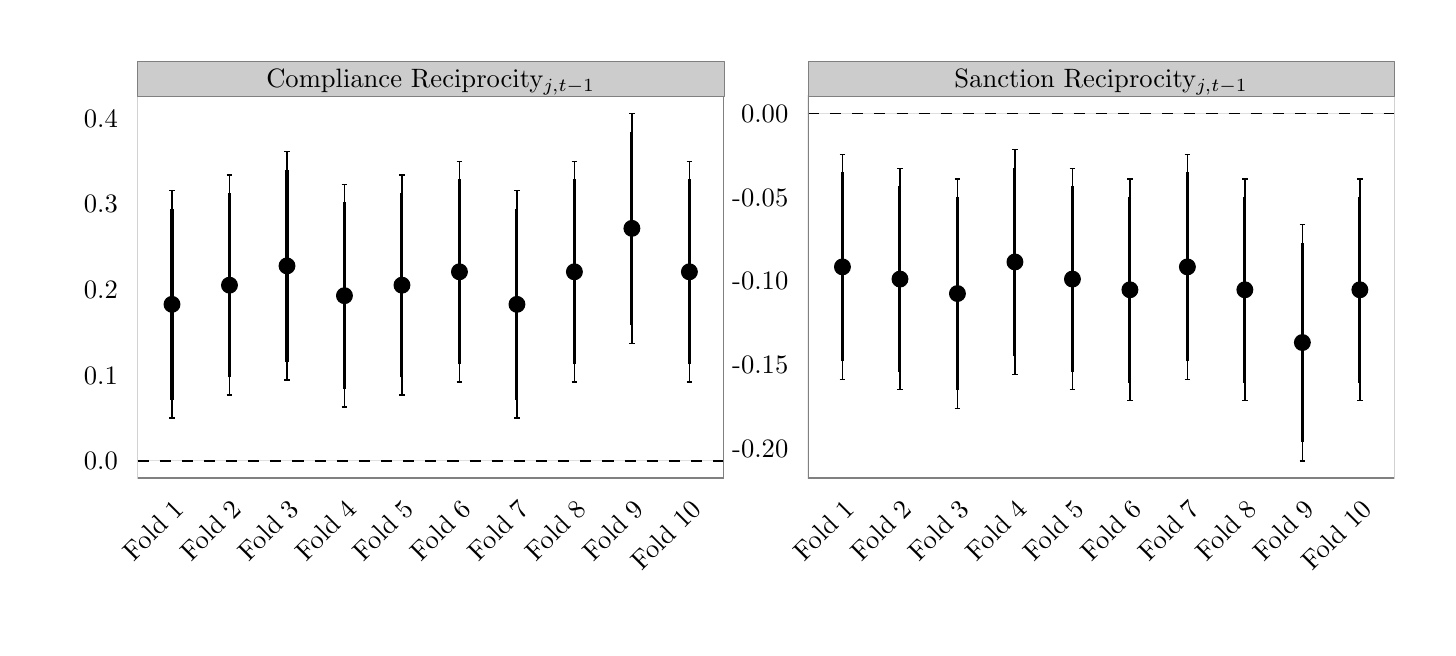
\begin{tikzpicture}[x=1pt,y=1pt]
\definecolor[named]{fillColor}{rgb}{1.00,1.00,1.00}
\path[use as bounding box,fill=fillColor,fill opacity=0.00] (0,0) rectangle (505.89,216.81);
\begin{scope}
\path[clip] (  0.00,  0.00) rectangle (505.89,216.81);
\definecolor[named]{drawColor}{rgb}{1.00,1.00,1.00}
\definecolor[named]{fillColor}{rgb}{1.00,1.00,1.00}

\path[draw=drawColor,line width= 0.6pt,line join=round,line cap=round,fill=fillColor] (  0.00,  0.00) rectangle (505.89,216.81);
\end{scope}
\begin{scope}
\path[clip] ( 39.69, 54.06) rectangle (251.57,192.13);
\definecolor[named]{fillColor}{rgb}{1.00,1.00,1.00}

\path[fill=fillColor] ( 39.69, 54.06) rectangle (251.57,192.13);
\definecolor[named]{drawColor}{rgb}{0.00,0.00,0.00}
\definecolor[named]{fillColor}{rgb}{0.00,0.00,0.00}

\path[draw=drawColor,draw opacity=0.30,line width= 0.3pt,line join=round,fill=fillColor,fill opacity=0.30] ( 52.15, 75.74) -- ( 52.15,157.92);

\path[draw=drawColor,draw opacity=0.30,line width= 0.3pt,line join=round,fill=fillColor,fill opacity=0.30] ( 72.92, 84.07) -- ( 72.92,163.46);

\path[draw=drawColor,draw opacity=0.30,line width= 0.3pt,line join=round,fill=fillColor,fill opacity=0.30] ( 93.70, 89.44) -- ( 93.70,172.01);

\path[draw=drawColor,draw opacity=0.30,line width= 0.3pt,line join=round,fill=fillColor,fill opacity=0.30] (114.47, 79.77) -- (114.47,160.16);

\path[draw=drawColor,draw opacity=0.30,line width= 0.3pt,line join=round,fill=fillColor,fill opacity=0.30] (135.24, 84.07) -- (135.24,163.46);

\path[draw=drawColor,draw opacity=0.30,line width= 0.3pt,line join=round,fill=fillColor,fill opacity=0.30] (156.02, 88.71) -- (156.02,168.47);

\path[draw=drawColor,draw opacity=0.30,line width= 0.3pt,line join=round,fill=fillColor,fill opacity=0.30] (176.79, 75.74) -- (176.79,157.92);

\path[draw=drawColor,draw opacity=0.30,line width= 0.3pt,line join=round,fill=fillColor,fill opacity=0.30] (197.56, 88.71) -- (197.56,168.47);

\path[draw=drawColor,draw opacity=0.30,line width= 0.3pt,line join=round,fill=fillColor,fill opacity=0.30] (218.34,102.73) -- (218.34,185.85);

\path[draw=drawColor,draw opacity=0.30,line width= 0.3pt,line join=round,fill=fillColor,fill opacity=0.30] (239.11, 88.71) -- (239.11,168.47);
\definecolor[named]{drawColor}{rgb}{0.00,0.00,0.00}
\definecolor[named]{fillColor}{rgb}{0.00,0.00,0.00}

\path[draw=drawColor,line width= 1.1pt,line join=round,fill=fillColor] ( 52.15, 82.35) -- ( 52.15,151.32);

\path[draw=drawColor,line width= 1.1pt,line join=round,fill=fillColor] ( 72.92, 90.45) -- ( 72.92,157.08);

\path[draw=drawColor,line width= 1.1pt,line join=round,fill=fillColor] ( 93.70, 96.08) -- ( 93.70,165.38);

\path[draw=drawColor,line width= 1.1pt,line join=round,fill=fillColor] (114.47, 86.24) -- (114.47,153.70);

\path[draw=drawColor,line width= 1.1pt,line join=round,fill=fillColor] (135.24, 90.45) -- (135.24,157.08);

\path[draw=drawColor,line width= 1.1pt,line join=round,fill=fillColor] (156.02, 95.12) -- (156.02,162.06);

\path[draw=drawColor,line width= 1.1pt,line join=round,fill=fillColor] (176.79, 82.35) -- (176.79,151.32);

\path[draw=drawColor,line width= 1.1pt,line join=round,fill=fillColor] (197.56, 95.12) -- (197.56,162.06);

\path[draw=drawColor,line width= 1.1pt,line join=round,fill=fillColor] (218.34,109.41) -- (218.34,179.17);

\path[draw=drawColor,line width= 1.1pt,line join=round,fill=fillColor] (239.11, 95.12) -- (239.11,162.06);

\path[draw=drawColor,line width= 0.6pt,dash pattern=on 4pt off 4pt ,line join=round,fill=fillColor] ( 39.69, 60.34) -- (251.57, 60.34);

\path[draw=drawColor,line width= 0.4pt,line join=round,line cap=round,fill=fillColor] ( 52.15,116.83) circle (  2.85);

\path[draw=drawColor,line width= 0.4pt,line join=round,line cap=round,fill=fillColor] ( 72.92,123.76) circle (  2.85);

\path[draw=drawColor,line width= 0.4pt,line join=round,line cap=round,fill=fillColor] ( 93.70,130.73) circle (  2.85);

\path[draw=drawColor,line width= 0.4pt,line join=round,line cap=round,fill=fillColor] (114.47,119.97) circle (  2.85);

\path[draw=drawColor,line width= 0.4pt,line join=round,line cap=round,fill=fillColor] (135.24,123.76) circle (  2.85);

\path[draw=drawColor,line width= 0.4pt,line join=round,line cap=round,fill=fillColor] (156.02,128.59) circle (  2.85);

\path[draw=drawColor,line width= 0.4pt,line join=round,line cap=round,fill=fillColor] (176.79,116.83) circle (  2.85);

\path[draw=drawColor,line width= 0.4pt,line join=round,line cap=round,fill=fillColor] (197.56,128.59) circle (  2.85);

\path[draw=drawColor,line width= 0.4pt,line join=round,line cap=round,fill=fillColor] (218.34,144.29) circle (  2.85);

\path[draw=drawColor,line width= 0.4pt,line join=round,line cap=round,fill=fillColor] (239.11,128.59) circle (  2.85);

\path[draw=drawColor,line width= 0.6pt,line join=round] ( 51.11,157.92) --
	( 53.19,157.92);

\path[draw=drawColor,line width= 0.6pt,line join=round] ( 52.15,157.92) --
	( 52.15, 75.74);

\path[draw=drawColor,line width= 0.6pt,line join=round] ( 51.11, 75.74) --
	( 53.19, 75.74);

\path[draw=drawColor,line width= 0.6pt,line join=round] ( 71.88,163.46) --
	( 73.96,163.46);

\path[draw=drawColor,line width= 0.6pt,line join=round] ( 72.92,163.46) --
	( 72.92, 84.07);

\path[draw=drawColor,line width= 0.6pt,line join=round] ( 71.88, 84.07) --
	( 73.96, 84.07);

\path[draw=drawColor,line width= 0.6pt,line join=round] ( 92.66,172.01) --
	( 94.74,172.01);

\path[draw=drawColor,line width= 0.6pt,line join=round] ( 93.70,172.01) --
	( 93.70, 89.44);

\path[draw=drawColor,line width= 0.6pt,line join=round] ( 92.66, 89.44) --
	( 94.74, 89.44);

\path[draw=drawColor,line width= 0.6pt,line join=round] (113.43,160.16) --
	(115.51,160.16);

\path[draw=drawColor,line width= 0.6pt,line join=round] (114.47,160.16) --
	(114.47, 79.77);

\path[draw=drawColor,line width= 0.6pt,line join=round] (113.43, 79.77) --
	(115.51, 79.77);

\path[draw=drawColor,line width= 0.6pt,line join=round] (134.20,163.46) --
	(136.28,163.46);

\path[draw=drawColor,line width= 0.6pt,line join=round] (135.24,163.46) --
	(135.24, 84.07);

\path[draw=drawColor,line width= 0.6pt,line join=round] (134.20, 84.07) --
	(136.28, 84.07);

\path[draw=drawColor,line width= 0.6pt,line join=round] (154.98,168.47) --
	(157.05,168.47);

\path[draw=drawColor,line width= 0.6pt,line join=round] (156.02,168.47) --
	(156.02, 88.71);

\path[draw=drawColor,line width= 0.6pt,line join=round] (154.98, 88.71) --
	(157.05, 88.71);

\path[draw=drawColor,line width= 0.6pt,line join=round] (175.75,157.92) --
	(177.83,157.92);

\path[draw=drawColor,line width= 0.6pt,line join=round] (176.79,157.92) --
	(176.79, 75.74);

\path[draw=drawColor,line width= 0.6pt,line join=round] (175.75, 75.74) --
	(177.83, 75.74);

\path[draw=drawColor,line width= 0.6pt,line join=round] (196.52,168.47) --
	(198.60,168.47);

\path[draw=drawColor,line width= 0.6pt,line join=round] (197.56,168.47) --
	(197.56, 88.71);

\path[draw=drawColor,line width= 0.6pt,line join=round] (196.52, 88.71) --
	(198.60, 88.71);

\path[draw=drawColor,line width= 0.6pt,line join=round] (217.30,185.85) --
	(219.37,185.85);

\path[draw=drawColor,line width= 0.6pt,line join=round] (218.34,185.85) --
	(218.34,102.73);

\path[draw=drawColor,line width= 0.6pt,line join=round] (217.30,102.73) --
	(219.37,102.73);

\path[draw=drawColor,line width= 0.6pt,line join=round] (238.07,168.47) --
	(240.15,168.47);

\path[draw=drawColor,line width= 0.6pt,line join=round] (239.11,168.47) --
	(239.11, 88.71);

\path[draw=drawColor,line width= 0.6pt,line join=round] (238.07, 88.71) --
	(240.15, 88.71);
\definecolor[named]{drawColor}{rgb}{0.50,0.50,0.50}

\path[draw=drawColor,line width= 0.6pt,line join=round,line cap=round] ( 39.69, 54.06) rectangle (251.57,192.13);
\end{scope}
\begin{scope}
\path[clip] (281.96, 54.06) rectangle (493.85,192.13);
\definecolor[named]{fillColor}{rgb}{1.00,1.00,1.00}

\path[fill=fillColor] (281.96, 54.06) rectangle (493.85,192.13);
\definecolor[named]{drawColor}{rgb}{0.00,0.00,0.00}
\definecolor[named]{fillColor}{rgb}{0.00,0.00,0.00}

\path[draw=drawColor,draw opacity=0.30,line width= 0.3pt,line join=round,fill=fillColor,fill opacity=0.30] (294.42, 89.70) -- (294.42,171.03);

\path[draw=drawColor,draw opacity=0.30,line width= 0.3pt,line join=round,fill=fillColor,fill opacity=0.30] (315.20, 86.01) -- (315.20,165.92);

\path[draw=drawColor,draw opacity=0.30,line width= 0.3pt,line join=round,fill=fillColor,fill opacity=0.30] (335.97, 79.21) -- (335.97,162.24);

\path[draw=drawColor,draw opacity=0.30,line width= 0.3pt,line join=round,fill=fillColor,fill opacity=0.30] (356.74, 91.50) -- (356.74,172.81);

\path[draw=drawColor,draw opacity=0.30,line width= 0.3pt,line join=round,fill=fillColor,fill opacity=0.30] (377.52, 86.01) -- (377.52,165.92);

\path[draw=drawColor,draw opacity=0.30,line width= 0.3pt,line join=round,fill=fillColor,fill opacity=0.30] (398.29, 82.11) -- (398.29,162.07);

\path[draw=drawColor,draw opacity=0.30,line width= 0.3pt,line join=round,fill=fillColor,fill opacity=0.30] (419.06, 89.70) -- (419.06,171.03);

\path[draw=drawColor,draw opacity=0.30,line width= 0.3pt,line join=round,fill=fillColor,fill opacity=0.30] (439.83, 82.11) -- (439.83,162.07);

\path[draw=drawColor,draw opacity=0.30,line width= 0.3pt,line join=round,fill=fillColor,fill opacity=0.30] (460.61, 60.34) -- (460.61,145.72);

\path[draw=drawColor,draw opacity=0.30,line width= 0.3pt,line join=round,fill=fillColor,fill opacity=0.30] (481.38, 82.11) -- (481.38,162.07);
\definecolor[named]{drawColor}{rgb}{0.00,0.00,0.00}
\definecolor[named]{fillColor}{rgb}{0.00,0.00,0.00}

\path[draw=drawColor,line width= 1.1pt,line join=round,fill=fillColor] (294.42, 96.24) -- (294.42,164.49);

\path[draw=drawColor,line width= 1.1pt,line join=round,fill=fillColor] (315.20, 92.43) -- (315.20,159.49);

\path[draw=drawColor,line width= 1.1pt,line join=round,fill=fillColor] (335.97, 85.89) -- (335.97,155.56);

\path[draw=drawColor,line width= 1.1pt,line join=round,fill=fillColor] (356.74, 98.04) -- (356.74,166.27);

\path[draw=drawColor,line width= 1.1pt,line join=round,fill=fillColor] (377.52, 92.43) -- (377.52,159.49);

\path[draw=drawColor,line width= 1.1pt,line join=round,fill=fillColor] (398.29, 88.54) -- (398.29,155.64);

\path[draw=drawColor,line width= 1.1pt,line join=round,fill=fillColor] (419.06, 96.24) -- (419.06,164.49);

\path[draw=drawColor,line width= 1.1pt,line join=round,fill=fillColor] (439.83, 88.54) -- (439.83,155.64);

\path[draw=drawColor,line width= 1.1pt,line join=round,fill=fillColor] (460.61, 67.20) -- (460.61,138.86);

\path[draw=drawColor,line width= 1.1pt,line join=round,fill=fillColor] (481.38, 88.54) -- (481.38,155.64);

\path[draw=drawColor,line width= 0.6pt,dash pattern=on 4pt off 4pt ,line join=round,fill=fillColor] (281.96,185.85) -- (493.85,185.85);

\path[draw=drawColor,line width= 0.4pt,line join=round,line cap=round,fill=fillColor] (294.42,130.37) circle (  2.85);

\path[draw=drawColor,line width= 0.4pt,line join=round,line cap=round,fill=fillColor] (315.20,125.96) circle (  2.85);

\path[draw=drawColor,line width= 0.4pt,line join=round,line cap=round,fill=fillColor] (335.97,120.73) circle (  2.85);

\path[draw=drawColor,line width= 0.4pt,line join=round,line cap=round,fill=fillColor] (356.74,132.15) circle (  2.85);

\path[draw=drawColor,line width= 0.4pt,line join=round,line cap=round,fill=fillColor] (377.52,125.96) circle (  2.85);

\path[draw=drawColor,line width= 0.4pt,line join=round,line cap=round,fill=fillColor] (398.29,122.09) circle (  2.85);

\path[draw=drawColor,line width= 0.4pt,line join=round,line cap=round,fill=fillColor] (419.06,130.37) circle (  2.85);

\path[draw=drawColor,line width= 0.4pt,line join=round,line cap=round,fill=fillColor] (439.83,122.09) circle (  2.85);

\path[draw=drawColor,line width= 0.4pt,line join=round,line cap=round,fill=fillColor] (460.61,103.03) circle (  2.85);

\path[draw=drawColor,line width= 0.4pt,line join=round,line cap=round,fill=fillColor] (481.38,122.09) circle (  2.85);

\path[draw=drawColor,line width= 0.6pt,line join=round] (293.38,171.03) --
	(295.46,171.03);

\path[draw=drawColor,line width= 0.6pt,line join=round] (294.42,171.03) --
	(294.42, 89.70);

\path[draw=drawColor,line width= 0.6pt,line join=round] (293.38, 89.70) --
	(295.46, 89.70);

\path[draw=drawColor,line width= 0.6pt,line join=round] (314.16,165.92) --
	(316.23,165.92);

\path[draw=drawColor,line width= 0.6pt,line join=round] (315.20,165.92) --
	(315.20, 86.01);

\path[draw=drawColor,line width= 0.6pt,line join=round] (314.16, 86.01) --
	(316.23, 86.01);

\path[draw=drawColor,line width= 0.6pt,line join=round] (334.93,162.24) --
	(337.01,162.24);

\path[draw=drawColor,line width= 0.6pt,line join=round] (335.97,162.24) --
	(335.97, 79.21);

\path[draw=drawColor,line width= 0.6pt,line join=round] (334.93, 79.21) --
	(337.01, 79.21);

\path[draw=drawColor,line width= 0.6pt,line join=round] (355.70,172.81) --
	(357.78,172.81);

\path[draw=drawColor,line width= 0.6pt,line join=round] (356.74,172.81) --
	(356.74, 91.50);

\path[draw=drawColor,line width= 0.6pt,line join=round] (355.70, 91.50) --
	(357.78, 91.50);

\path[draw=drawColor,line width= 0.6pt,line join=round] (376.48,165.92) --
	(378.55,165.92);

\path[draw=drawColor,line width= 0.6pt,line join=round] (377.52,165.92) --
	(377.52, 86.01);

\path[draw=drawColor,line width= 0.6pt,line join=round] (376.48, 86.01) --
	(378.55, 86.01);

\path[draw=drawColor,line width= 0.6pt,line join=round] (397.25,162.07) --
	(399.33,162.07);

\path[draw=drawColor,line width= 0.6pt,line join=round] (398.29,162.07) --
	(398.29, 82.11);

\path[draw=drawColor,line width= 0.6pt,line join=round] (397.25, 82.11) --
	(399.33, 82.11);

\path[draw=drawColor,line width= 0.6pt,line join=round] (418.02,171.03) --
	(420.10,171.03);

\path[draw=drawColor,line width= 0.6pt,line join=round] (419.06,171.03) --
	(419.06, 89.70);

\path[draw=drawColor,line width= 0.6pt,line join=round] (418.02, 89.70) --
	(420.10, 89.70);

\path[draw=drawColor,line width= 0.6pt,line join=round] (438.80,162.07) --
	(440.87,162.07);

\path[draw=drawColor,line width= 0.6pt,line join=round] (439.83,162.07) --
	(439.83, 82.11);

\path[draw=drawColor,line width= 0.6pt,line join=round] (438.80, 82.11) --
	(440.87, 82.11);

\path[draw=drawColor,line width= 0.6pt,line join=round] (459.57,145.72) --
	(461.65,145.72);

\path[draw=drawColor,line width= 0.6pt,line join=round] (460.61,145.72) --
	(460.61, 60.34);

\path[draw=drawColor,line width= 0.6pt,line join=round] (459.57, 60.34) --
	(461.65, 60.34);

\path[draw=drawColor,line width= 0.6pt,line join=round] (480.34,162.07) --
	(482.42,162.07);

\path[draw=drawColor,line width= 0.6pt,line join=round] (481.38,162.07) --
	(481.38, 82.11);

\path[draw=drawColor,line width= 0.6pt,line join=round] (480.34, 82.11) --
	(482.42, 82.11);
\definecolor[named]{drawColor}{rgb}{0.50,0.50,0.50}

\path[draw=drawColor,line width= 0.6pt,line join=round,line cap=round] (281.96, 54.06) rectangle (493.85,192.13);
\end{scope}
\begin{scope}
\path[clip] (  0.00,  0.00) rectangle (505.89,216.81);
\definecolor[named]{drawColor}{rgb}{0.50,0.50,0.50}
\definecolor[named]{fillColor}{rgb}{0.80,0.80,0.80}

\path[draw=drawColor,line width= 0.2pt,line join=round,line cap=round,fill=fillColor] ( 39.69,192.13) rectangle (251.57,204.77);
\definecolor[named]{drawColor}{rgb}{0.00,0.00,0.00}

\node[text=drawColor,anchor=base,inner sep=0pt, outer sep=0pt, scale=  0.96] at (145.63,195.14) {Compliance Reciprocity$_{j,t-1}$};
\end{scope}
\begin{scope}
\path[clip] (  0.00,  0.00) rectangle (505.89,216.81);
\definecolor[named]{drawColor}{rgb}{0.50,0.50,0.50}
\definecolor[named]{fillColor}{rgb}{0.80,0.80,0.80}

\path[draw=drawColor,line width= 0.2pt,line join=round,line cap=round,fill=fillColor] (281.96,192.13) rectangle (493.85,204.77);
\definecolor[named]{drawColor}{rgb}{0.00,0.00,0.00}

\node[text=drawColor,anchor=base,inner sep=0pt, outer sep=0pt, scale=  0.96] at (387.90,195.14) {Sanction Reciprocity$_{j,t-1}$};
\end{scope}
\begin{scope}
\path[clip] (  0.00,  0.00) rectangle (505.89,216.81);
\definecolor[named]{drawColor}{rgb}{0.00,0.00,0.00}

\node[text=drawColor,anchor=base east,inner sep=0pt, outer sep=0pt, scale=  0.96] at ( 32.57, 57.03) {0.0};

\node[text=drawColor,anchor=base east,inner sep=0pt, outer sep=0pt, scale=  0.96] at ( 32.57, 88.00) {0.1};

\node[text=drawColor,anchor=base east,inner sep=0pt, outer sep=0pt, scale=  0.96] at ( 32.57,118.97) {0.2};

\node[text=drawColor,anchor=base east,inner sep=0pt, outer sep=0pt, scale=  0.96] at ( 32.57,149.94) {0.3};

\node[text=drawColor,anchor=base east,inner sep=0pt, outer sep=0pt, scale=  0.96] at ( 32.57,180.91) {0.4};
\end{scope}
\begin{scope}
\path[clip] (  0.00,  0.00) rectangle (505.89,216.81);
\definecolor[named]{drawColor}{rgb}{0.00,0.00,0.00}

\node[text=drawColor,anchor=base east,inner sep=0pt, outer sep=0pt, scale=  0.96] at (274.85, 61.51) {-0.20};

\node[text=drawColor,anchor=base east,inner sep=0pt, outer sep=0pt, scale=  0.96] at (274.85, 91.77) {-0.15};

\node[text=drawColor,anchor=base east,inner sep=0pt, outer sep=0pt, scale=  0.96] at (274.85,122.03) {-0.10};

\node[text=drawColor,anchor=base east,inner sep=0pt, outer sep=0pt, scale=  0.96] at (274.85,152.29) {-0.05};

\node[text=drawColor,anchor=base east,inner sep=0pt, outer sep=0pt, scale=  0.96] at (274.85,182.55) {0.00};
\end{scope}
\begin{scope}
\path[clip] (  0.00,  0.00) rectangle (505.89,216.81);
\definecolor[named]{drawColor}{rgb}{0.00,0.00,0.00}

\node[text=drawColor,rotate= 45.00,anchor=base east,inner sep=0pt, outer sep=0pt, scale=  0.96] at ( 56.83, 42.27) {Fold 1};

\node[text=drawColor,rotate= 45.00,anchor=base east,inner sep=0pt, outer sep=0pt, scale=  0.96] at ( 77.60, 42.27) {Fold 2};

\node[text=drawColor,rotate= 45.00,anchor=base east,inner sep=0pt, outer sep=0pt, scale=  0.96] at ( 98.37, 42.27) {Fold 3};

\node[text=drawColor,rotate= 45.00,anchor=base east,inner sep=0pt, outer sep=0pt, scale=  0.96] at (119.15, 42.27) {Fold 4};

\node[text=drawColor,rotate= 45.00,anchor=base east,inner sep=0pt, outer sep=0pt, scale=  0.96] at (139.92, 42.27) {Fold 5};

\node[text=drawColor,rotate= 45.00,anchor=base east,inner sep=0pt, outer sep=0pt, scale=  0.96] at (160.69, 42.27) {Fold 6};

\node[text=drawColor,rotate= 45.00,anchor=base east,inner sep=0pt, outer sep=0pt, scale=  0.96] at (181.46, 42.27) {Fold 7};

\node[text=drawColor,rotate= 45.00,anchor=base east,inner sep=0pt, outer sep=0pt, scale=  0.96] at (202.24, 42.27) {Fold 8};

\node[text=drawColor,rotate= 45.00,anchor=base east,inner sep=0pt, outer sep=0pt, scale=  0.96] at (223.01, 42.27) {Fold 9};

\node[text=drawColor,rotate= 45.00,anchor=base east,inner sep=0pt, outer sep=0pt, scale=  0.96] at (243.78, 42.27) {Fold 10};
\end{scope}
\begin{scope}
\path[clip] (  0.00,  0.00) rectangle (505.89,216.81);
\definecolor[named]{drawColor}{rgb}{0.00,0.00,0.00}

\node[text=drawColor,rotate= 45.00,anchor=base east,inner sep=0pt, outer sep=0pt, scale=  0.96] at (299.10, 42.27) {Fold 1};

\node[text=drawColor,rotate= 45.00,anchor=base east,inner sep=0pt, outer sep=0pt, scale=  0.96] at (319.87, 42.27) {Fold 2};

\node[text=drawColor,rotate= 45.00,anchor=base east,inner sep=0pt, outer sep=0pt, scale=  0.96] at (340.64, 42.27) {Fold 3};

\node[text=drawColor,rotate= 45.00,anchor=base east,inner sep=0pt, outer sep=0pt, scale=  0.96] at (361.42, 42.27) {Fold 4};

\node[text=drawColor,rotate= 45.00,anchor=base east,inner sep=0pt, outer sep=0pt, scale=  0.96] at (382.19, 42.27) {Fold 5};

\node[text=drawColor,rotate= 45.00,anchor=base east,inner sep=0pt, outer sep=0pt, scale=  0.96] at (402.96, 42.27) {Fold 6};

\node[text=drawColor,rotate= 45.00,anchor=base east,inner sep=0pt, outer sep=0pt, scale=  0.96] at (423.74, 42.27) {Fold 7};

\node[text=drawColor,rotate= 45.00,anchor=base east,inner sep=0pt, outer sep=0pt, scale=  0.96] at (444.51, 42.27) {Fold 8};

\node[text=drawColor,rotate= 45.00,anchor=base east,inner sep=0pt, outer sep=0pt, scale=  0.96] at (465.28, 42.27) {Fold 9};

\node[text=drawColor,rotate= 45.00,anchor=base east,inner sep=0pt, outer sep=0pt, scale=  0.96] at (486.06, 42.27) {Fold 10};
\end{scope}
\end{tikzpicture}
